\documentclass{article}

\usepackage[utf8]{inputenc}		% obsluga jezyka polskiego
\usepackage[MeX]{polski}		%

\usepackage[top=1in, bottom=1.25in, left=1.25in, right=1.25in]{geometry}		%zmiana marginesów

\usepackage{graphicx}		%wyswietlanie obrazow
\usepackage{float}			%

\usepackage{rotating}		%obracanie obrazow
\usepackage{tikz}			%

\usepackage{multicol}		%tekst w kolumnach

\usepackage{listings}											%obsluga wyswietlania kodu
\usepackage{xcolor}												%
\lstset { %														%
	basicstyle=\ttfamily    									%
    language=C,													%
    backgroundcolor=\color{black!5}, % set backgroundcolor		%
    basicstyle=\footnotesize,% basic font setting				%
}																%

\renewcommand{\labelitemi}{--}			%zmiana wygladu znacznikow wypunktowania
\renewcommand{\labelitemii}{--}		%
%\usepackage[export]{adjustbox}

\begin{document}

\begin{titlepage} 
	\newcommand{\HRule}{\rule{\linewidth}{0.5mm}} 
	
	\center 
	
	%------------------------------------------------
	%	Headings
	%------------------------------------------------
	
	\textsc{\LARGE Politechnika Wrocławska}\\[1.5cm] % Main heading such as the name of your university/college
	
	%\textsc{\Large Podstawy Techniki Mikroprocesorowej}\\[0.5cm] % Major heading such as course name
	
	%\textsc{\large Dokumentacja techniczna projektu}\\[0.5cm] % Minor heading such as course title
	
	%------------------------------------------------
	%	Title
	%------------------------------------------------
	
	\HRule\\[0.4cm]
	
	{\huge\bfseries Przewodnik Elektroniczny}\\[0.4cm] % Title of your document
	
	\HRule\\[1.5cm]
	
	%------------------------------------------------
	%	Author(s)
	%------------------------------------------------
	
	%\begin{minipage}{0.5\textwidth}
	%	\begin{flushleft}
	%		\large
	%		\textit{Autor:}\\
	%		\textsc{Maciej Mielcarski} \\numer albumu: 235703\\~\\Wydział Elektroniki W-4\\Automatyka i Robotyka 
	%	\end{flushleft}
	%\end{minipage}
	%~
	%\begin{minipage}{0.4\textwidth}
	%	\begin{flushright}
	%		\large
	%		\textit{Grupa zajęciowa:}\\
	%		\textsc{ŚR TP 13:15} 
	%	\end{flushright}
	%\end{minipage}

\vfill\vfill\vfill % Position the date 3/4 down the remaining page
	
	{\large Maciej Mielcarski \\~\\15.04.2018 wersja projektu 1.0 } % Date, change the \today to a set date if you want to be precise 
	
\end{titlepage}



\pagenumbering{gobble}

  %\maketitle
  \newpage
\pagenumbering{arabic}  

\section{Wstęp}
lorem ipsum
\section{Atmel AVR}
Avr lorem ipsum
\subsection{Atmega 8}
atmega 9 lorem ipsum

\begin{figure}[H]
	\center
	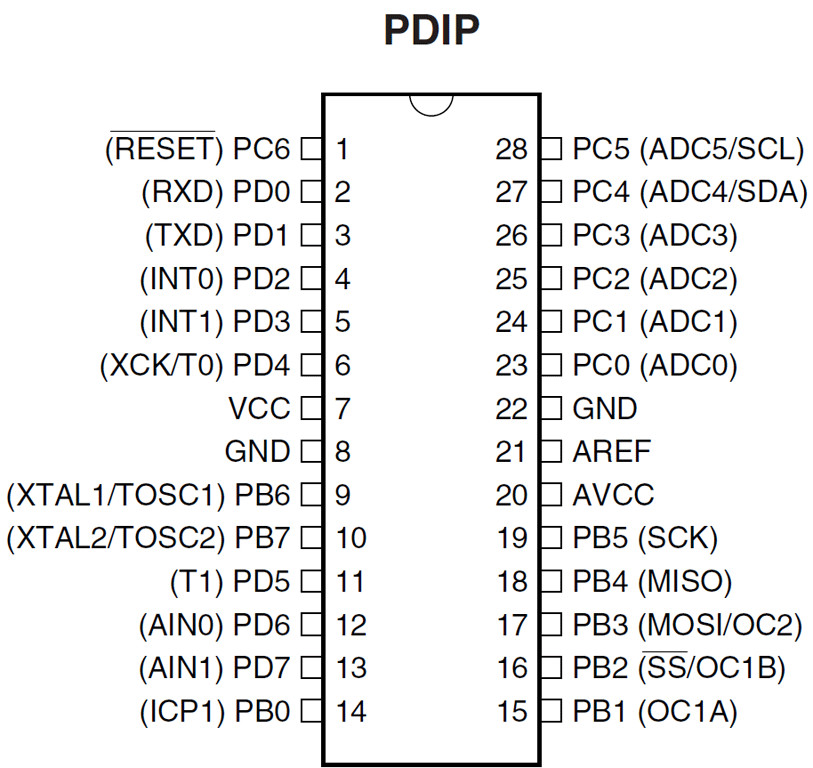
\includegraphics[width=\textwidth]{img/atmega8-pinout.jpg}
	\caption{Atmega 8 wyprowadzenia}
	\label{fig:img1}
\end{figure}

\subsection{Atmega 32}
atmega 32 lorem ipsum

\begin{figure}[H]
	\center
	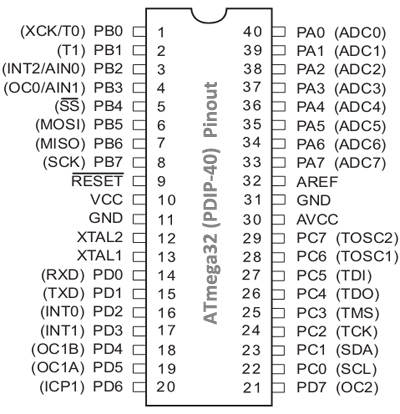
\includegraphics[width=\textwidth]{img/atmega32-pinout.jpg}
	\caption{Atmega 32 wyprowadzenia}
	\label{fig:img2}
\end{figure}

\subsection{Zasilanie}
zasilanie lorem ipsum

\begin{figure}[H]
	\center
	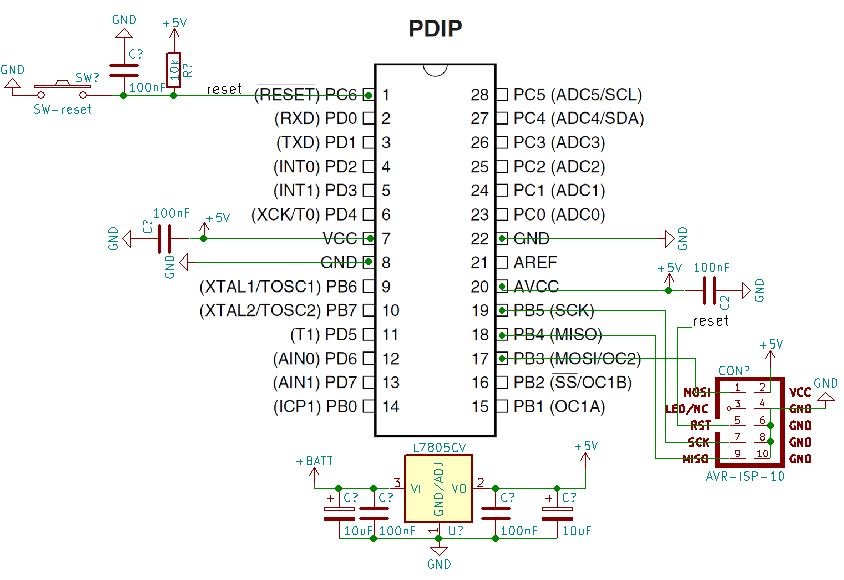
\includegraphics[width=\textwidth]{img/atmega-zasilanie.jpg}
	\caption{Atmega 8 zasilanie + programator}
	\label{fig:img3}
\end{figure}

\subsection{Programowanie}
\subsubsection{Makefile}

\subsection{Szablony programów}
\subsubsection{Kod bazowy}

\begin{figure}[H]
	\center
	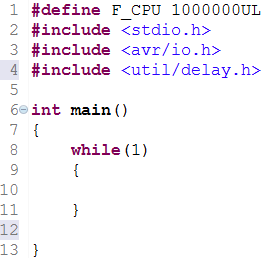
\includegraphics[scale=0.8]{img/kod-bazowy.jpg}
	\caption{Atmega kod bazowy w C}
	\label{fig:img4}
\end{figure}

\section{Podłączenie elementów wykonawczych}
\subsection{Eliminacja drgań styków - przycisk monostabilny}

\begin{figure}[H]
	\center
	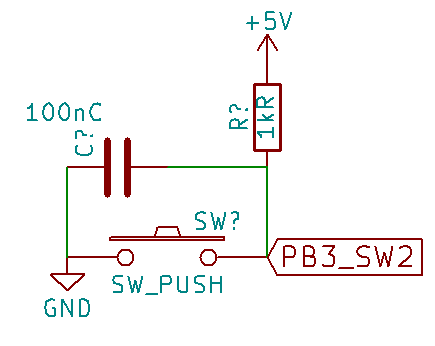
\includegraphics[scale=0.8]{img/przycisk-mono.jpg}
	\caption{kompensacja drgań styków przycisku monostabilnego}
	\label{fig:img5}
\end{figure}

\section{Arduino}
arduino lorem ipsum

\subsection{Arduino UNO}

\begin{figure}[H]
	\center
	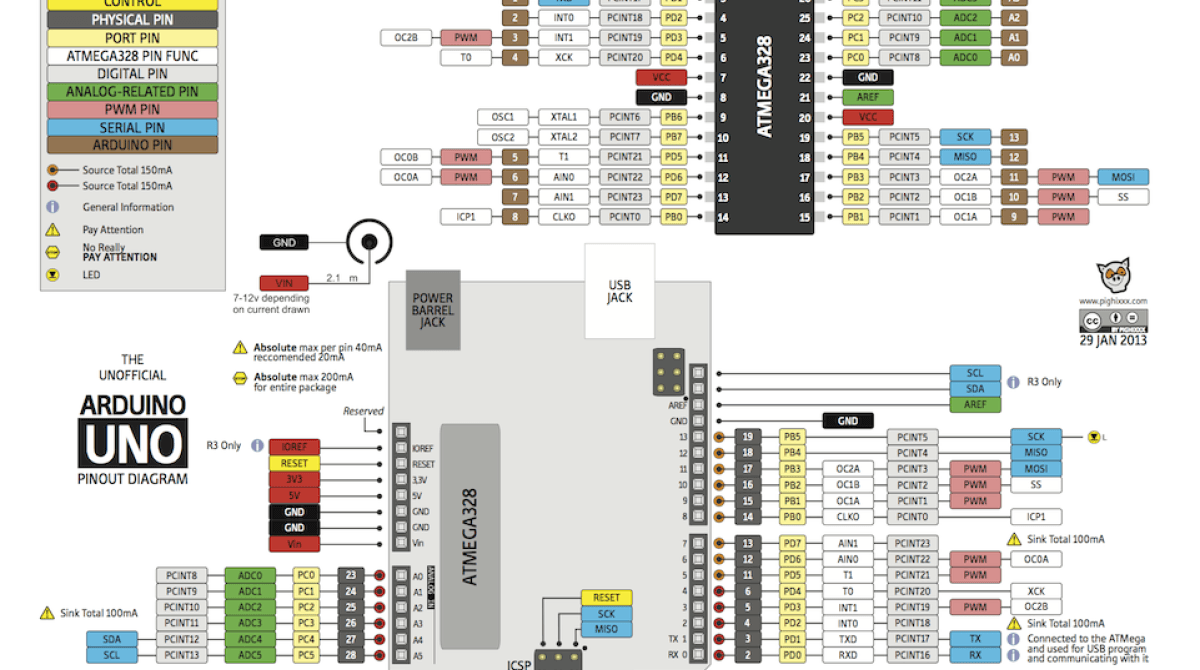
\includegraphics[scale=0.4]{img/arduino-pinout.png}
	\caption{arduino uno i atmega 328 - wyprowadzenia}
	\label{fig:img6}
\end{figure}

\begin{itemize}
	\item Arduino UNO:
\item mikrokontroler: 		ATmega328P
\item napięcie pracy: 			5V
\item napięcie zasilania: 		6-20V
\item wyjścia/wejścia cyfrowe: 	14 (w tym 6 PWM)
\item wejścia analogowe: 		6
\item wydajność prądowa pinu: 	20mA
\item pamięć Flash: 			32 KB 
\item pamięć SRAM: 			2KB
\item pamięć EEPROM: 		1KB
\item zegar: 				16 MHz
\item wymiary: 			68.6 x 53.4 mm, 25 g
\end{itemize}

\subsection{Obsługa bibliotek}
\subsubsection{Podstawowe operacje na pinach}

Biblioteka implementacji funkcji C++ : <Wire.h>\\
Obsługa pinów cyfrowych na przykładzie pinu nr 5:\\~\\

pinmode: 			pinMode(x, OUTPUT)\\
pullup				pinMode(x, INPUT\_PULLUP)\\
ustawianie stanu: 		digitalWrite(x,HIGH)\\
czytanie stanu: 			digitalRead(button)\\
opóźnienie: 			delay(50)\\

\section{Użytkowanie urządzenia}
Użytkownik obsługujący nadajnik Morse'a ma do dyspozycji szereg opcji związanych z nadawaniem i wyświetlaniem wiadomości. Interakcja z urządzeniem zachodzi poprzez obroty enkodera oraz 3 przyciski obsługujące zarówno długie jak i krótkie wciśnięcia.

\subsection{Menu główne}
Po uruchomieniu urządzenia użytkownikowi ukazuje się menu główne, obejmujące następujące pozycje:

\begin{itemize}
	\item	\textbf{nadaj}\newline
Opcja umozliwiająca wprowadzenie wiadomości za pośrednictwem obrotów enkodera oraz nadanie jej po wciśnięciu enkodera. Po skończeniu transmisji pojawia się komunikat pytający, czy powtórzyć nadawanie. Podczas transmisji wyświetlana jest sekwencja nadawanego kodu morse'a.

	\begin{itemize}
	\item uruchomienie opcji: wciśnięcie przycisku enkodera
	\item wybór znaku: obroty enkodera (zakres od a-z)
	\item zatwierdzenie znaku: wciśnięcie przycisku enkodera
	\item zatwierdzenie wiadomości: wciśnięcie przycisku enkodera przez co najmniej 2s
	\item powtórzenie nadawania: lewy lub prawy przycisk
	\end{itemize}

	\item	\textbf{wyswietl}\newline
Po wybraniu tej opcji, użytkownik ma okazję wyświetlić ostatnią nadaną przez niego wiadomość, zarówno w wersji znaków ASCII, jak i w kodzie morse'a. Za pomocą przycisków monostabilnych możliwe jest horyzontalne poruszanie się po wyświetlanej wiadomości. Wyjście z opcji przeglądania następuje po wciśnięciu przycisku enkodera.

	\begin{itemize}
	\item uruchomienie opcji: wciśnięcie przycisku enkodera
	\item przeglądanie wiadomości: lewy lub prawy przysik
	\item zakończenie opcji: wciśnięcie przycisku enkodera
	\end{itemize}

	\item	\textbf{rozszyf.}\newline
Jest to pozycja umożliwiająca wprowadzenie wiadomości w kodzie morse'a i przetworzenie jej na kod ASCII. Aktualnie nie jest dostępna, jednakże prace nad jej implementacją trwają.
	\item	\textbf{predk.}\newline
Za pomocą tej opcji możemy dostosować prędkość wyświetlanej przez nas wiadomości. Wartość ta wyrażana jest w słowach na minutę ( ang. wpm - words per minute), przy czym wartość 1 słowa na minutę oznacza prędkość wystarczającą do nadania słowa "PARIS" w ciągu jednej minuty (słowo "PARIS" zawira najbardziej standardowy przekrój liter w języku angielskim). Domyslnie, urządzenie nastawione jest na prędkość nadawania 10 wpm.

	\begin{itemize}
	\item uruchomienie opcji: wciśnięcie przycisku enkodera
	\item wybór prędkości: obroty enkodera
	\item zatwierdzenie prędkości: wciśnięcie przycisku enkodera
	\end{itemize}

\end{itemize}

\section{Kod programu}

\subsection{Główny pilk modułowy main.c}
\begin{multicols}{2}
\lstset{tabsize=1}
\begin{lstlisting}

\end{lstlisting}
\end{multicols}

\subsection{Plik modułowy morse.c}

\begin{multicols}{2}
\lstset{tabsize=1}
\begin{lstlisting}


\end{lstlisting}
%\columnbreak
\end{multicols}

\section{Dalszy rozwój projektu}
Mimo sprawnej realizacji większości planowanych funkcji urządzenia, układ daleki jest od finalnej wersji. Po skonstruowaniu i przetestowaniu podstawowych czynności, układ jest gotowy do implementacji kolejnych etapów rozwoju, m.in.:
	\begin{itemize}
	\item dokończenie pracy nad funkcją rozszyfrowywania wiadomości
	
	\item przerojektowanie programu w celu zaimplementowania obiektów, takich jak przyciski, enkoder, opcje menu jako struktury (stworzenie szablonów do elementów wykonawczych, znacząco ułatwiło by to budowę kolejnych projektów)
	
	\item wprowadzenie możliwości nadawania paru wyrazów, trwałego zapisywania wiadomości oraz zapętlania przekazu	
	
	\item zaprojektowanie płytki drukowanej PCB wraz z obsługą zasilania baterią Li-Ion
	
	\item przebudowanie całości projektu do formy poręcznej latarki
	\end{itemize}

\end{document}
